\chapter{Implementation and Experiments}

\begin{markdown}

This chapter describes the implementation of the experimental framework used in this thesis, including the selected tools and libraries, the integration of experiment tracking, and the methodology used for model training and evaluation.

\end{markdown}

\section{Used Tools and Libraries}

\begin{markdown}

The implementation developed in this thesis relies on several widely used machine learning and natural language processing libraries:

- MLflow -- an experiment tracking framework used for monitoring training runs, logging metrics, storing artifacts, and comparing model configurations through a graphical user interface.

- NLTK -- a natural language processing library used mainly for selected preprocessing operations and alternative tokenization approaches.

- Transformers -- the Hugging Face Transformers framework used for downloading, configuring, and training pretrained transformer-based models. All transformer architectures used in this thesis were implemented using this library.

- PyTorch -- the deep learning framework used as the computational backend for model training and inference.

- Pandas and NumPy -- libraries used for dataset manipulation, preprocessing, and general numerical operations.

\end{markdown}


\section{Integration with MLflow}

\begin{markdown}

MLflow is an open-source framework designed for experiment tracking and machine learning workflow management. Training transformer-based models typically requires a large number of experiments involving different preprocessing pipelines, hyperparameter configurations, and model architectures. In such scenarios, systematic tracking of experiments becomes important for reproducibility, comparison of results, and debugging.

In this thesis, MLflow was integrated into the training pipeline so that all experiments, metrics, parameters, and artifacts were automatically logged for later analysis.

The greatest advantage of MLflow is its support for debugging and experiment inspection. Training deep learning models is often computationally expensive and susceptible to implementation or preprocessing errors. Logging intermediate metrics and artifacts makes it easier to identify inconsistencies and detect potential problems during training.

\end{markdown}

\begin{figure}[h]
    \centering
    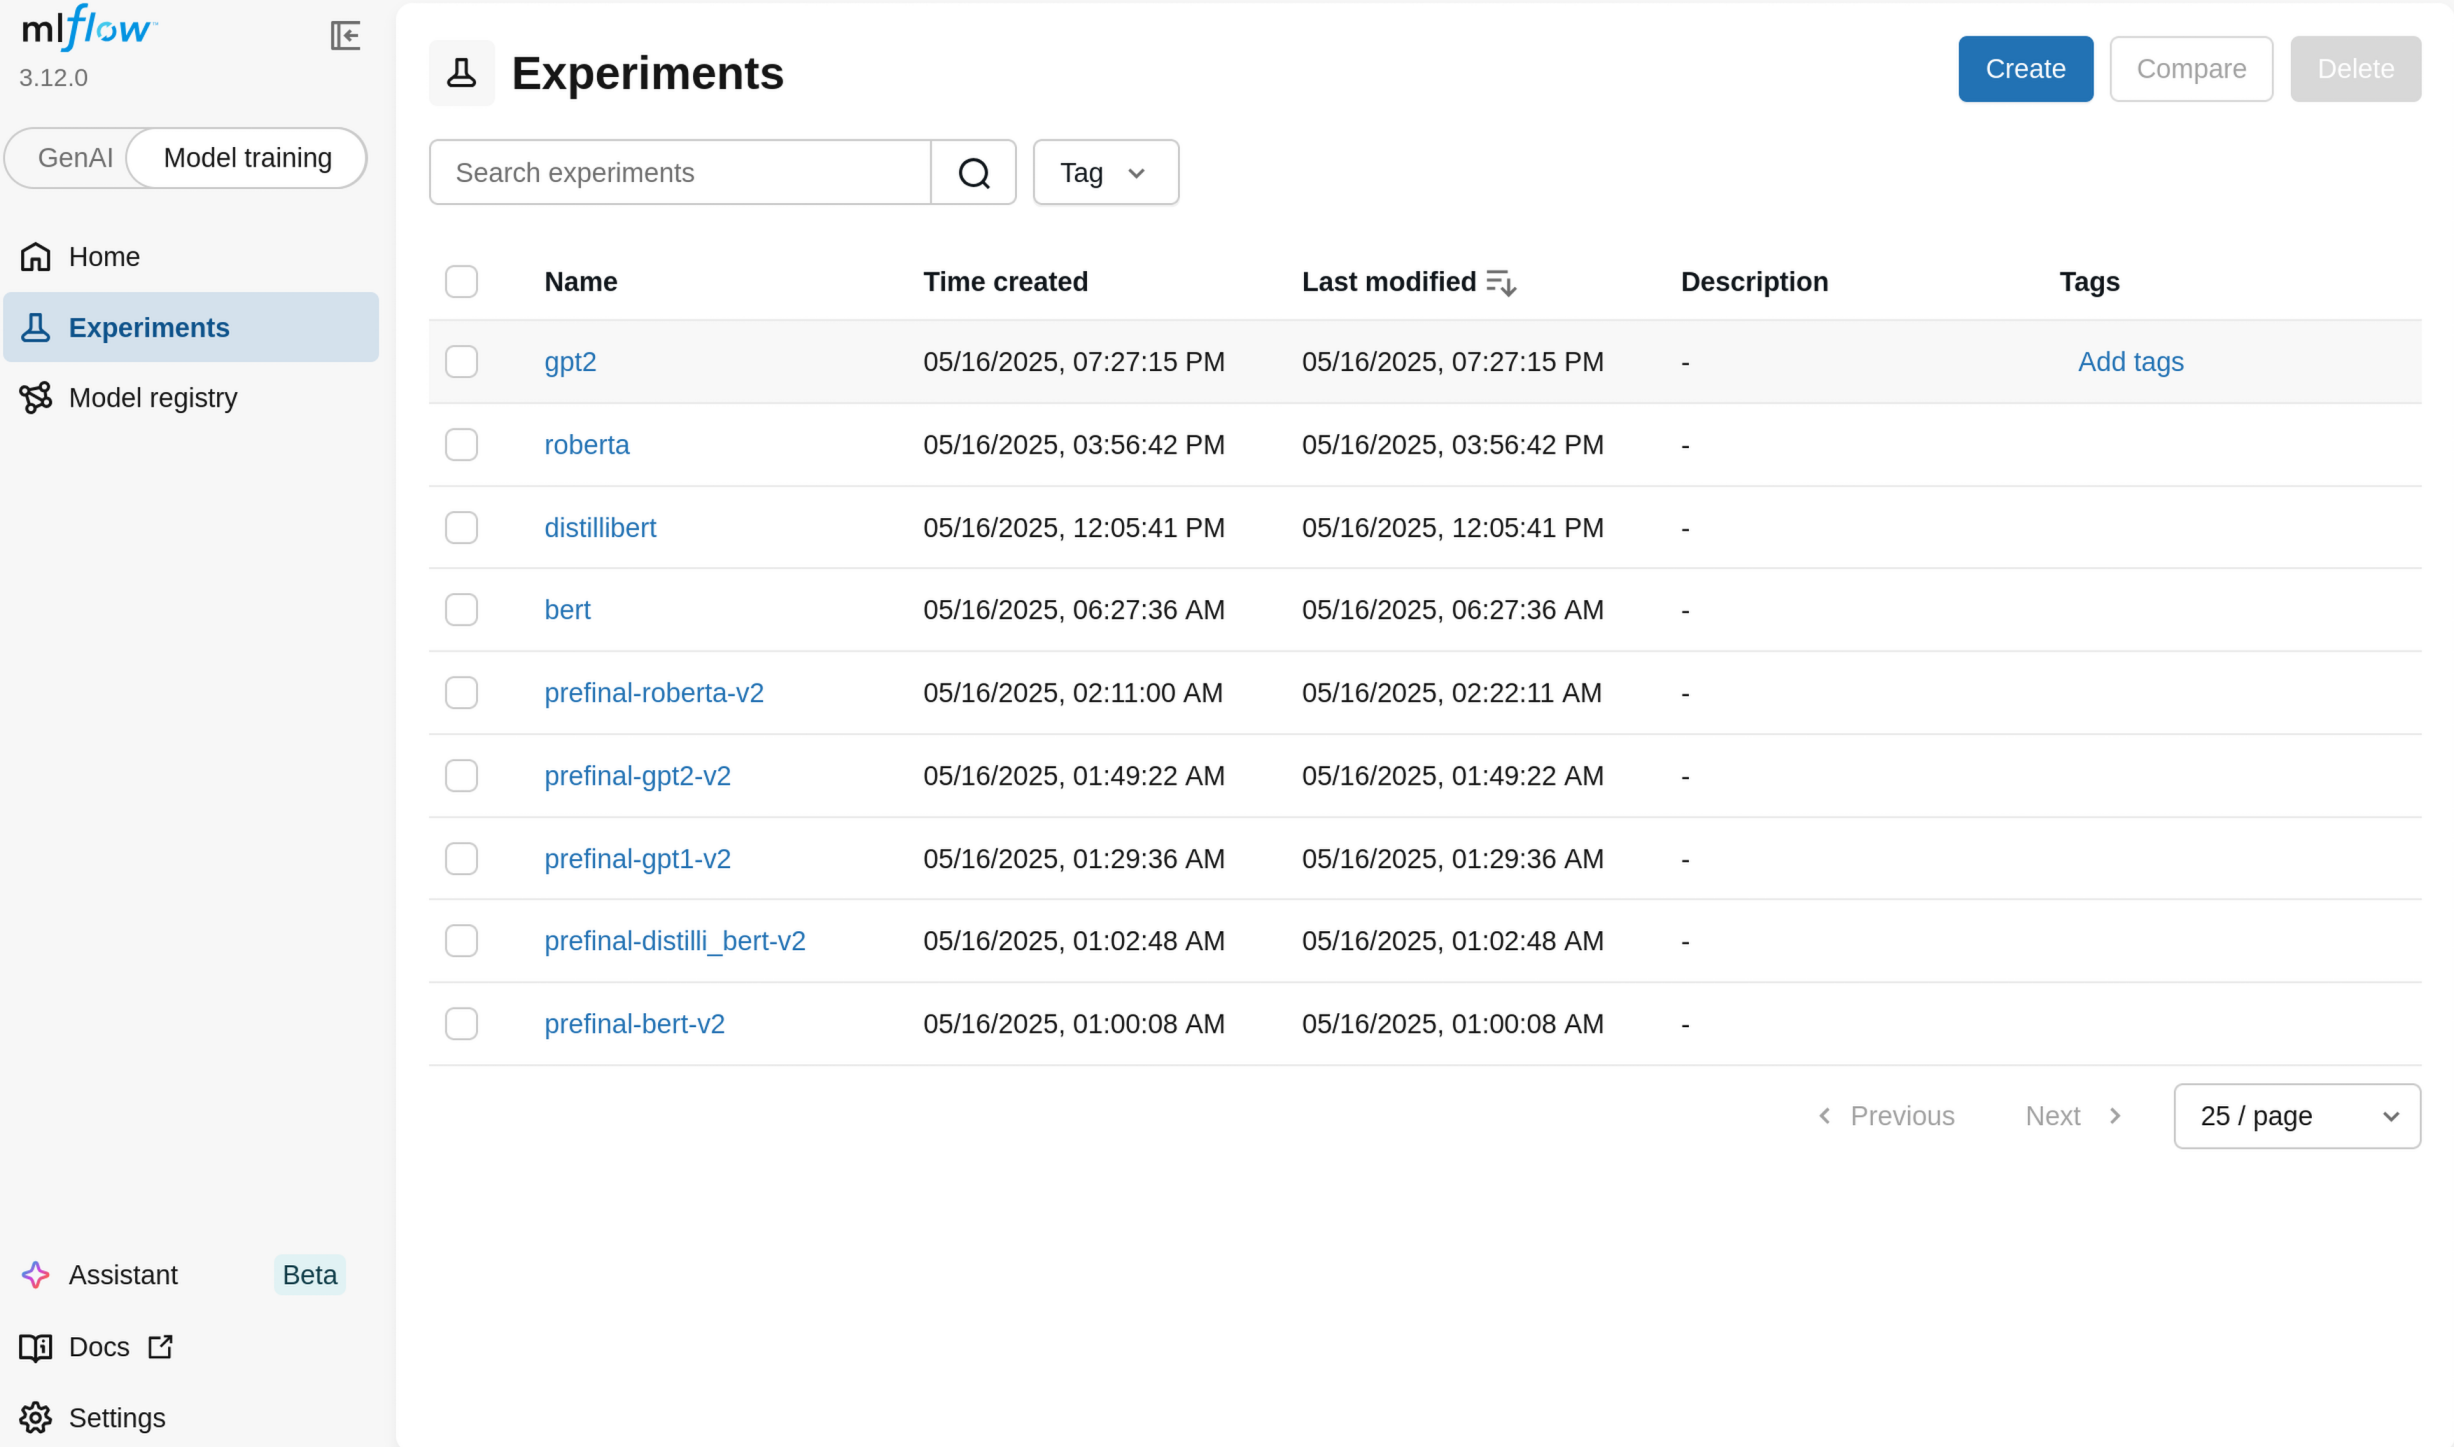
\includegraphics[width=\textwidth]{assets/mlflow_experiments.png}
    \caption{MLflow interface displaying recorded experiments}
    \label{fig:mlflow_experiments}
\end{figure}

\FloatBarrier

\begin{markdown}

Figure \ref{fig:mlflow_experiments} shows the MLflow experiment overview interface used during development. In this work, each transformer architecture was organized as a separate experiment, while individual runs within the experiment represented different hyperparameter configurations and preprocessing combinations.

\end{markdown}

\begin{figure}[h]
    \centering
    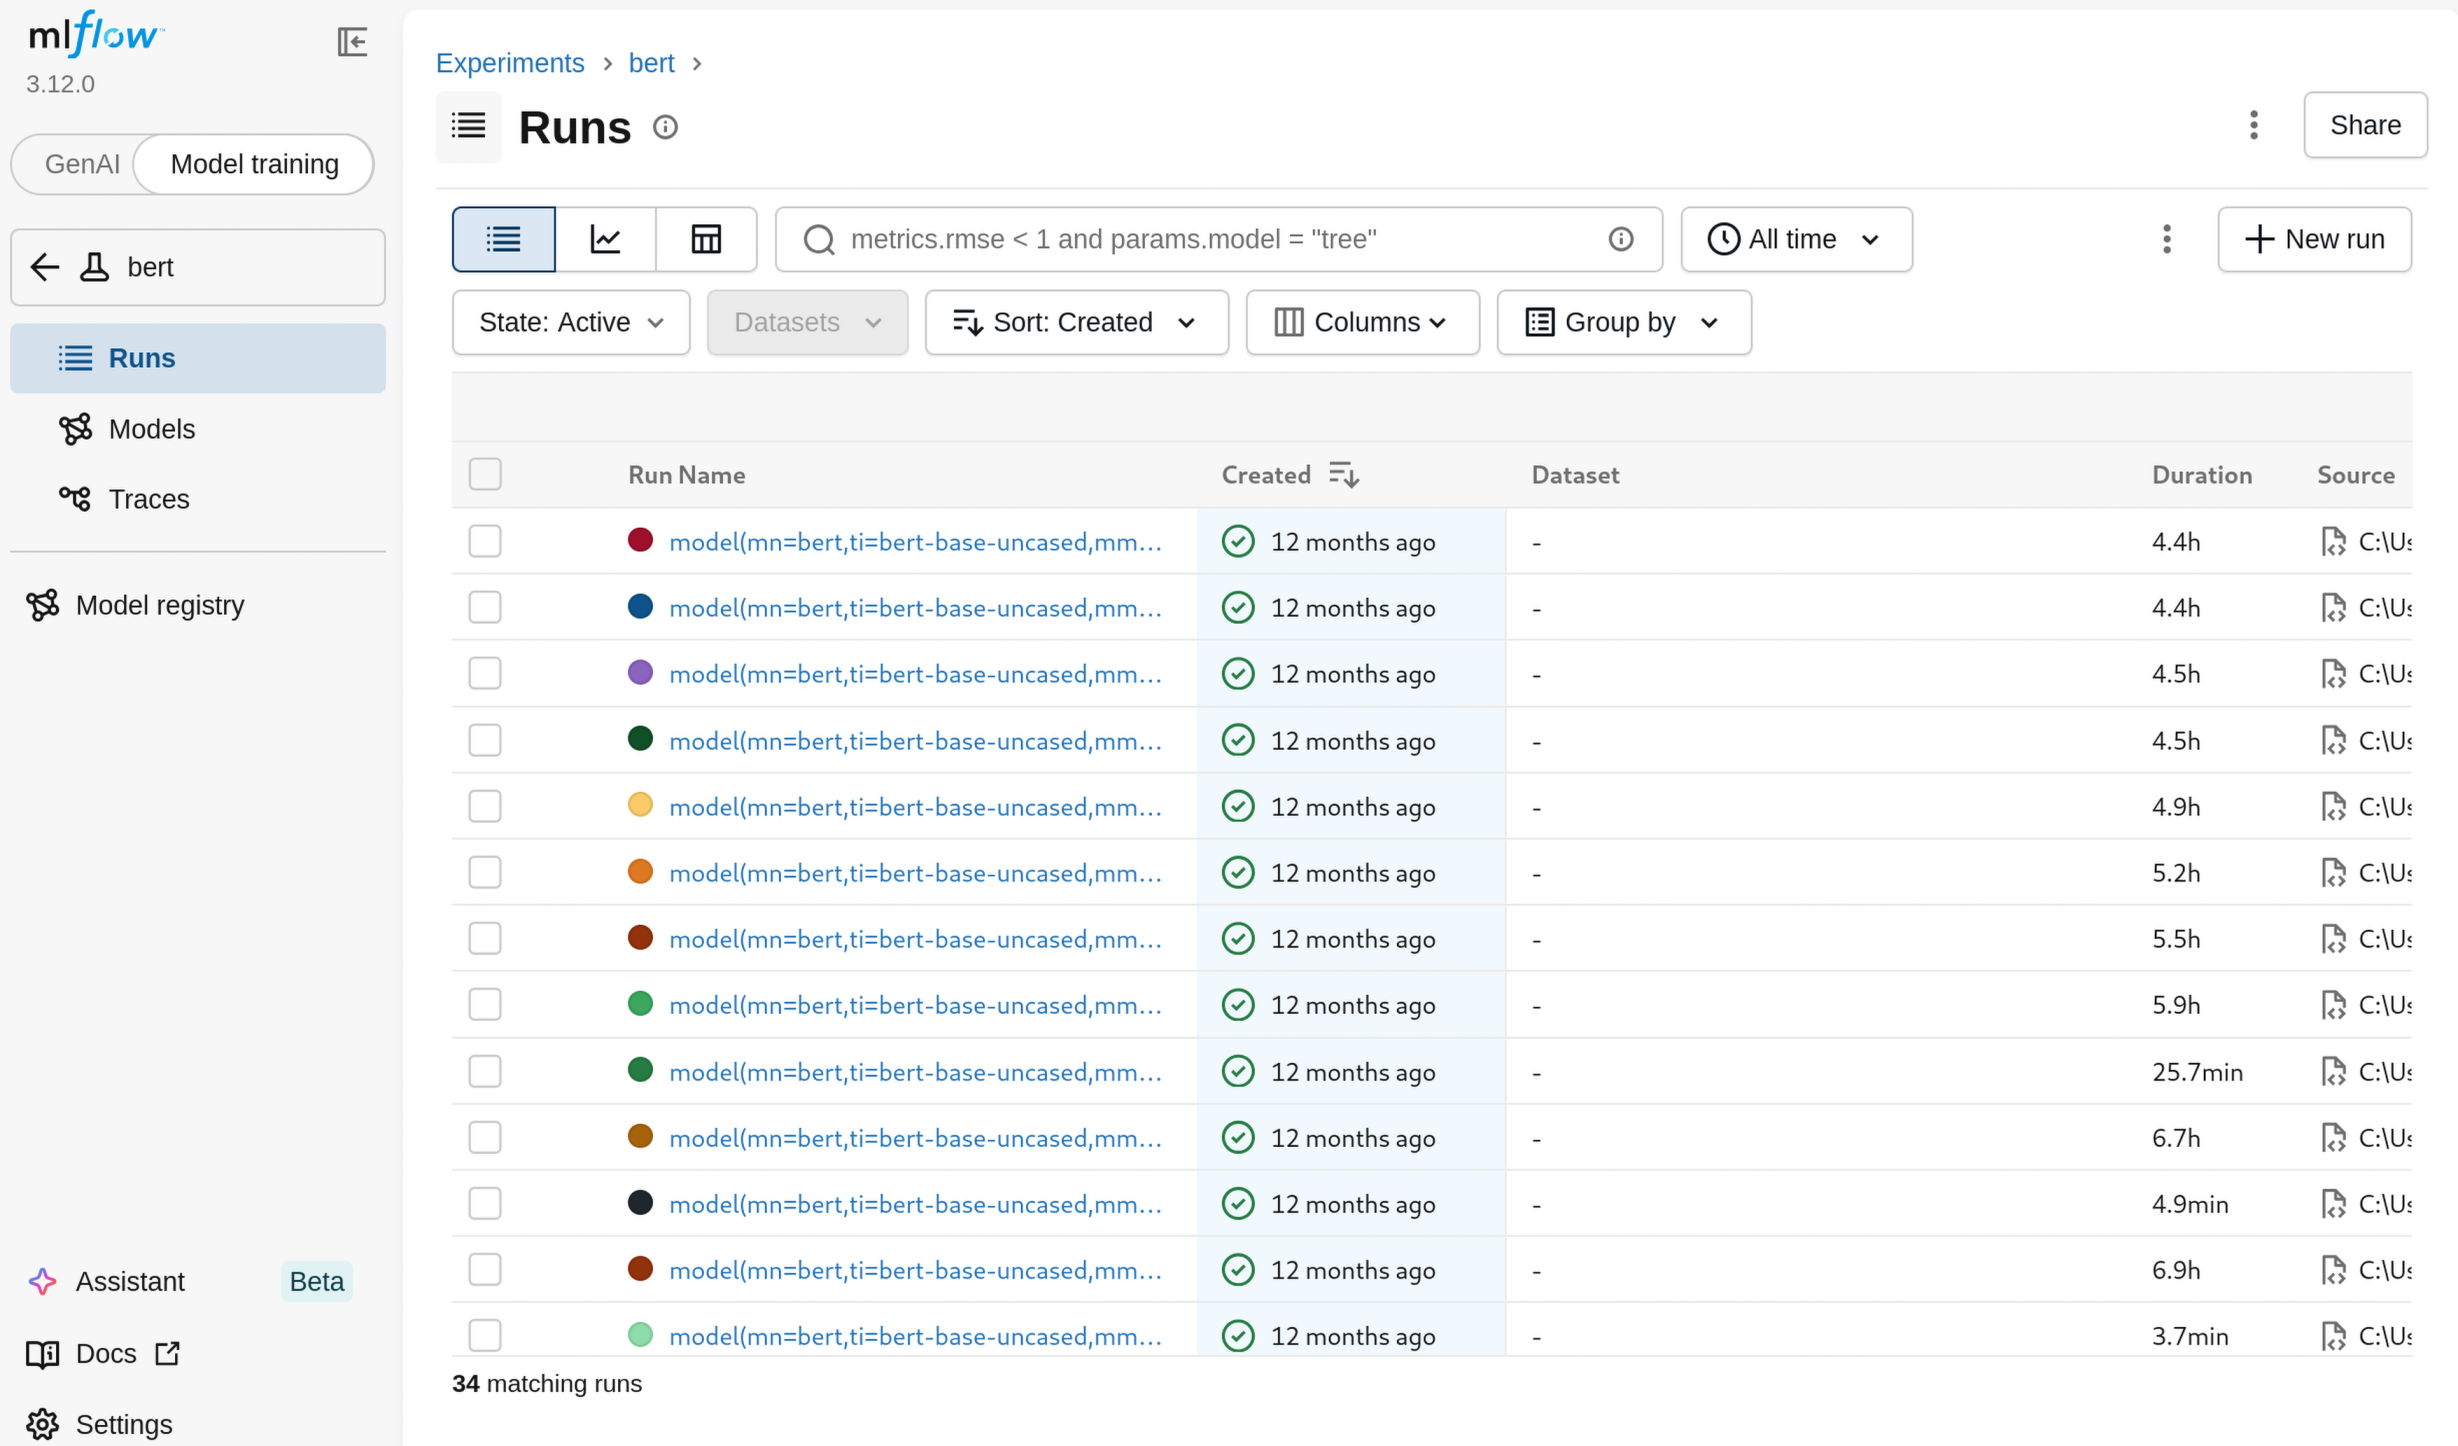
\includegraphics[width=\textwidth]{assets/mlflow_bert_runs.png}
    \caption{Recorded runs for the BERT experiment in MLflow}
    \label{fig:mlflow_bert_runs}
\end{figure}

\begin{markdown}

MLflow provides a flexible interface for tracking training metadata and allows customization of displayed parameters and metrics. Besides standard training statistics, additional information such as training duration and preprocessing configurations can also be recorded.

The framework also enables continuous monitoring of evaluation metrics during training, making it possible to analyze model behavior across epochs and identify unstable or problematic runs early in the experimentation process. Custom metrics can also be added directly from the training code when needed.

\end{markdown}

\begin{figure}[h]
    \centering
    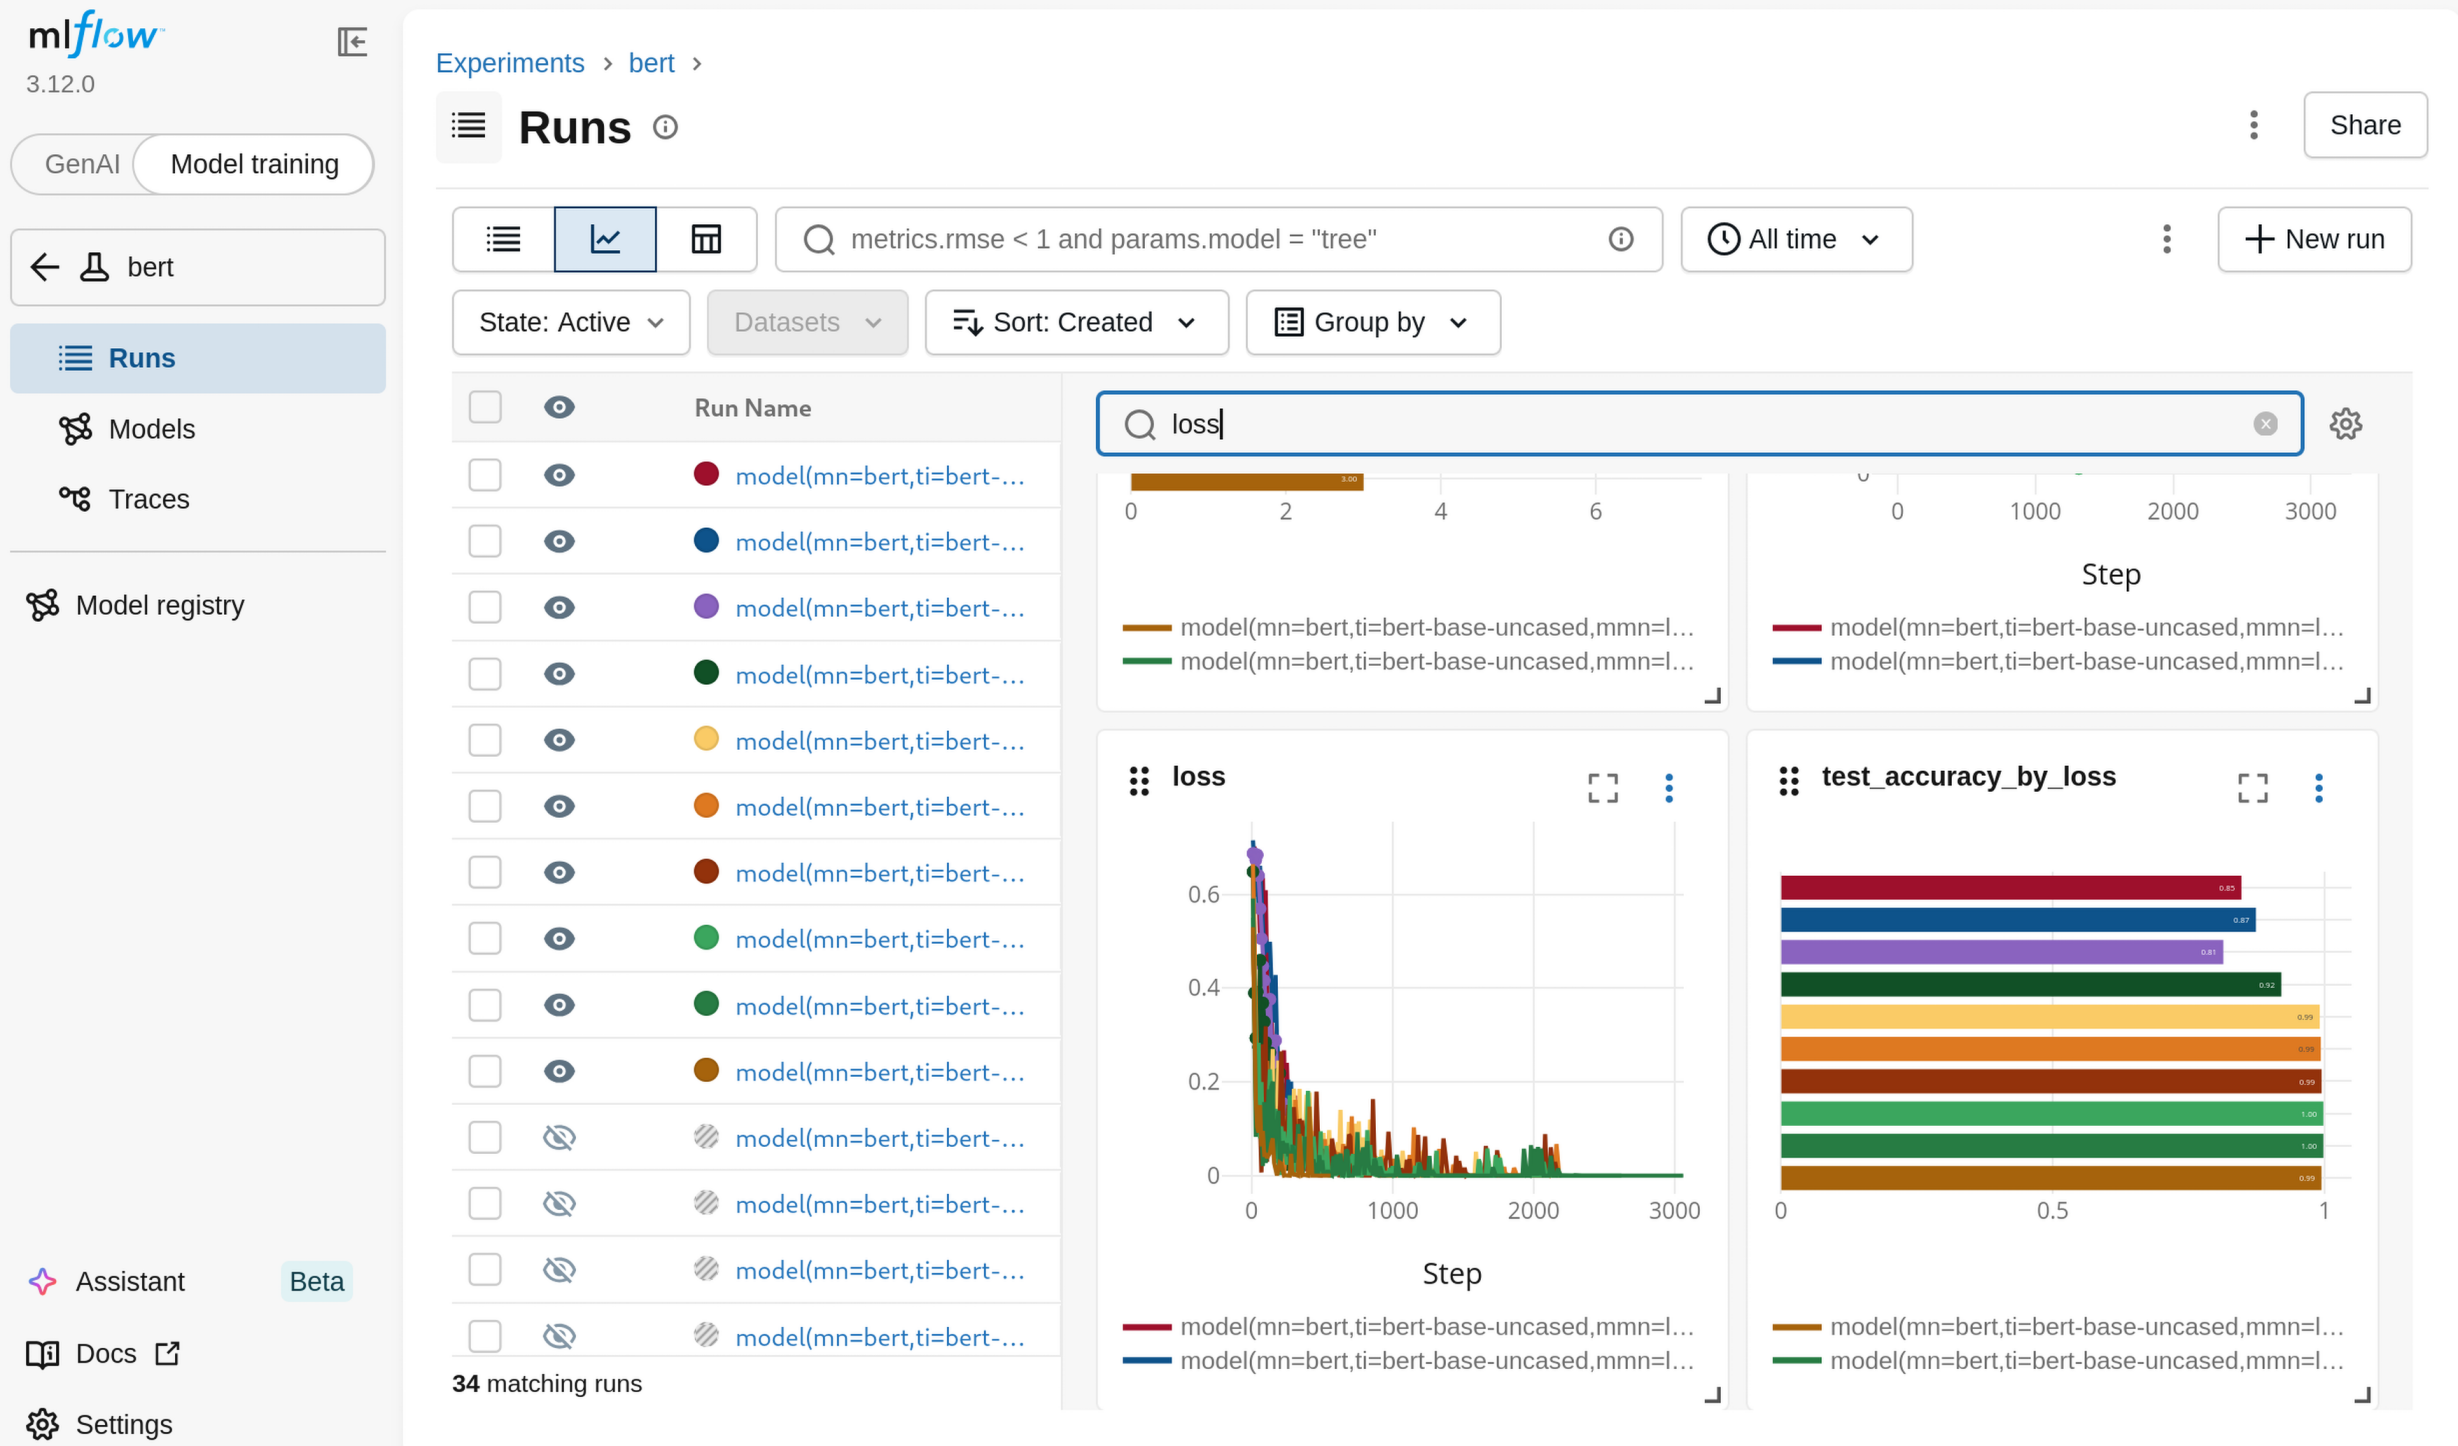
\includegraphics[width=\textwidth]{assets/mlflow_bert_run_metrics.png}
    \caption{Example of tracked training metrics in MLflow}
    \label{fig:mlflow_bert_run_metrics}
\end{figure}

\FloatBarrier

\begin{markdown}

Each experiment run additionally stores the corresponding training parameters and random seeds used during execution. Many parameters are logged automatically by the Transformers framework, while additional custom information can also be recorded manually. This setup improves experiment reproducibility.
Although full reproducibility is difficult to achieve in deep learning environments due to nondeterministic GPU operations and framework-level randomness, this work attempts to maximize reproducibility by consistently storing random seeds and experiment configurations.

\end{markdown}

\begin{figure}[h]
    \centering
    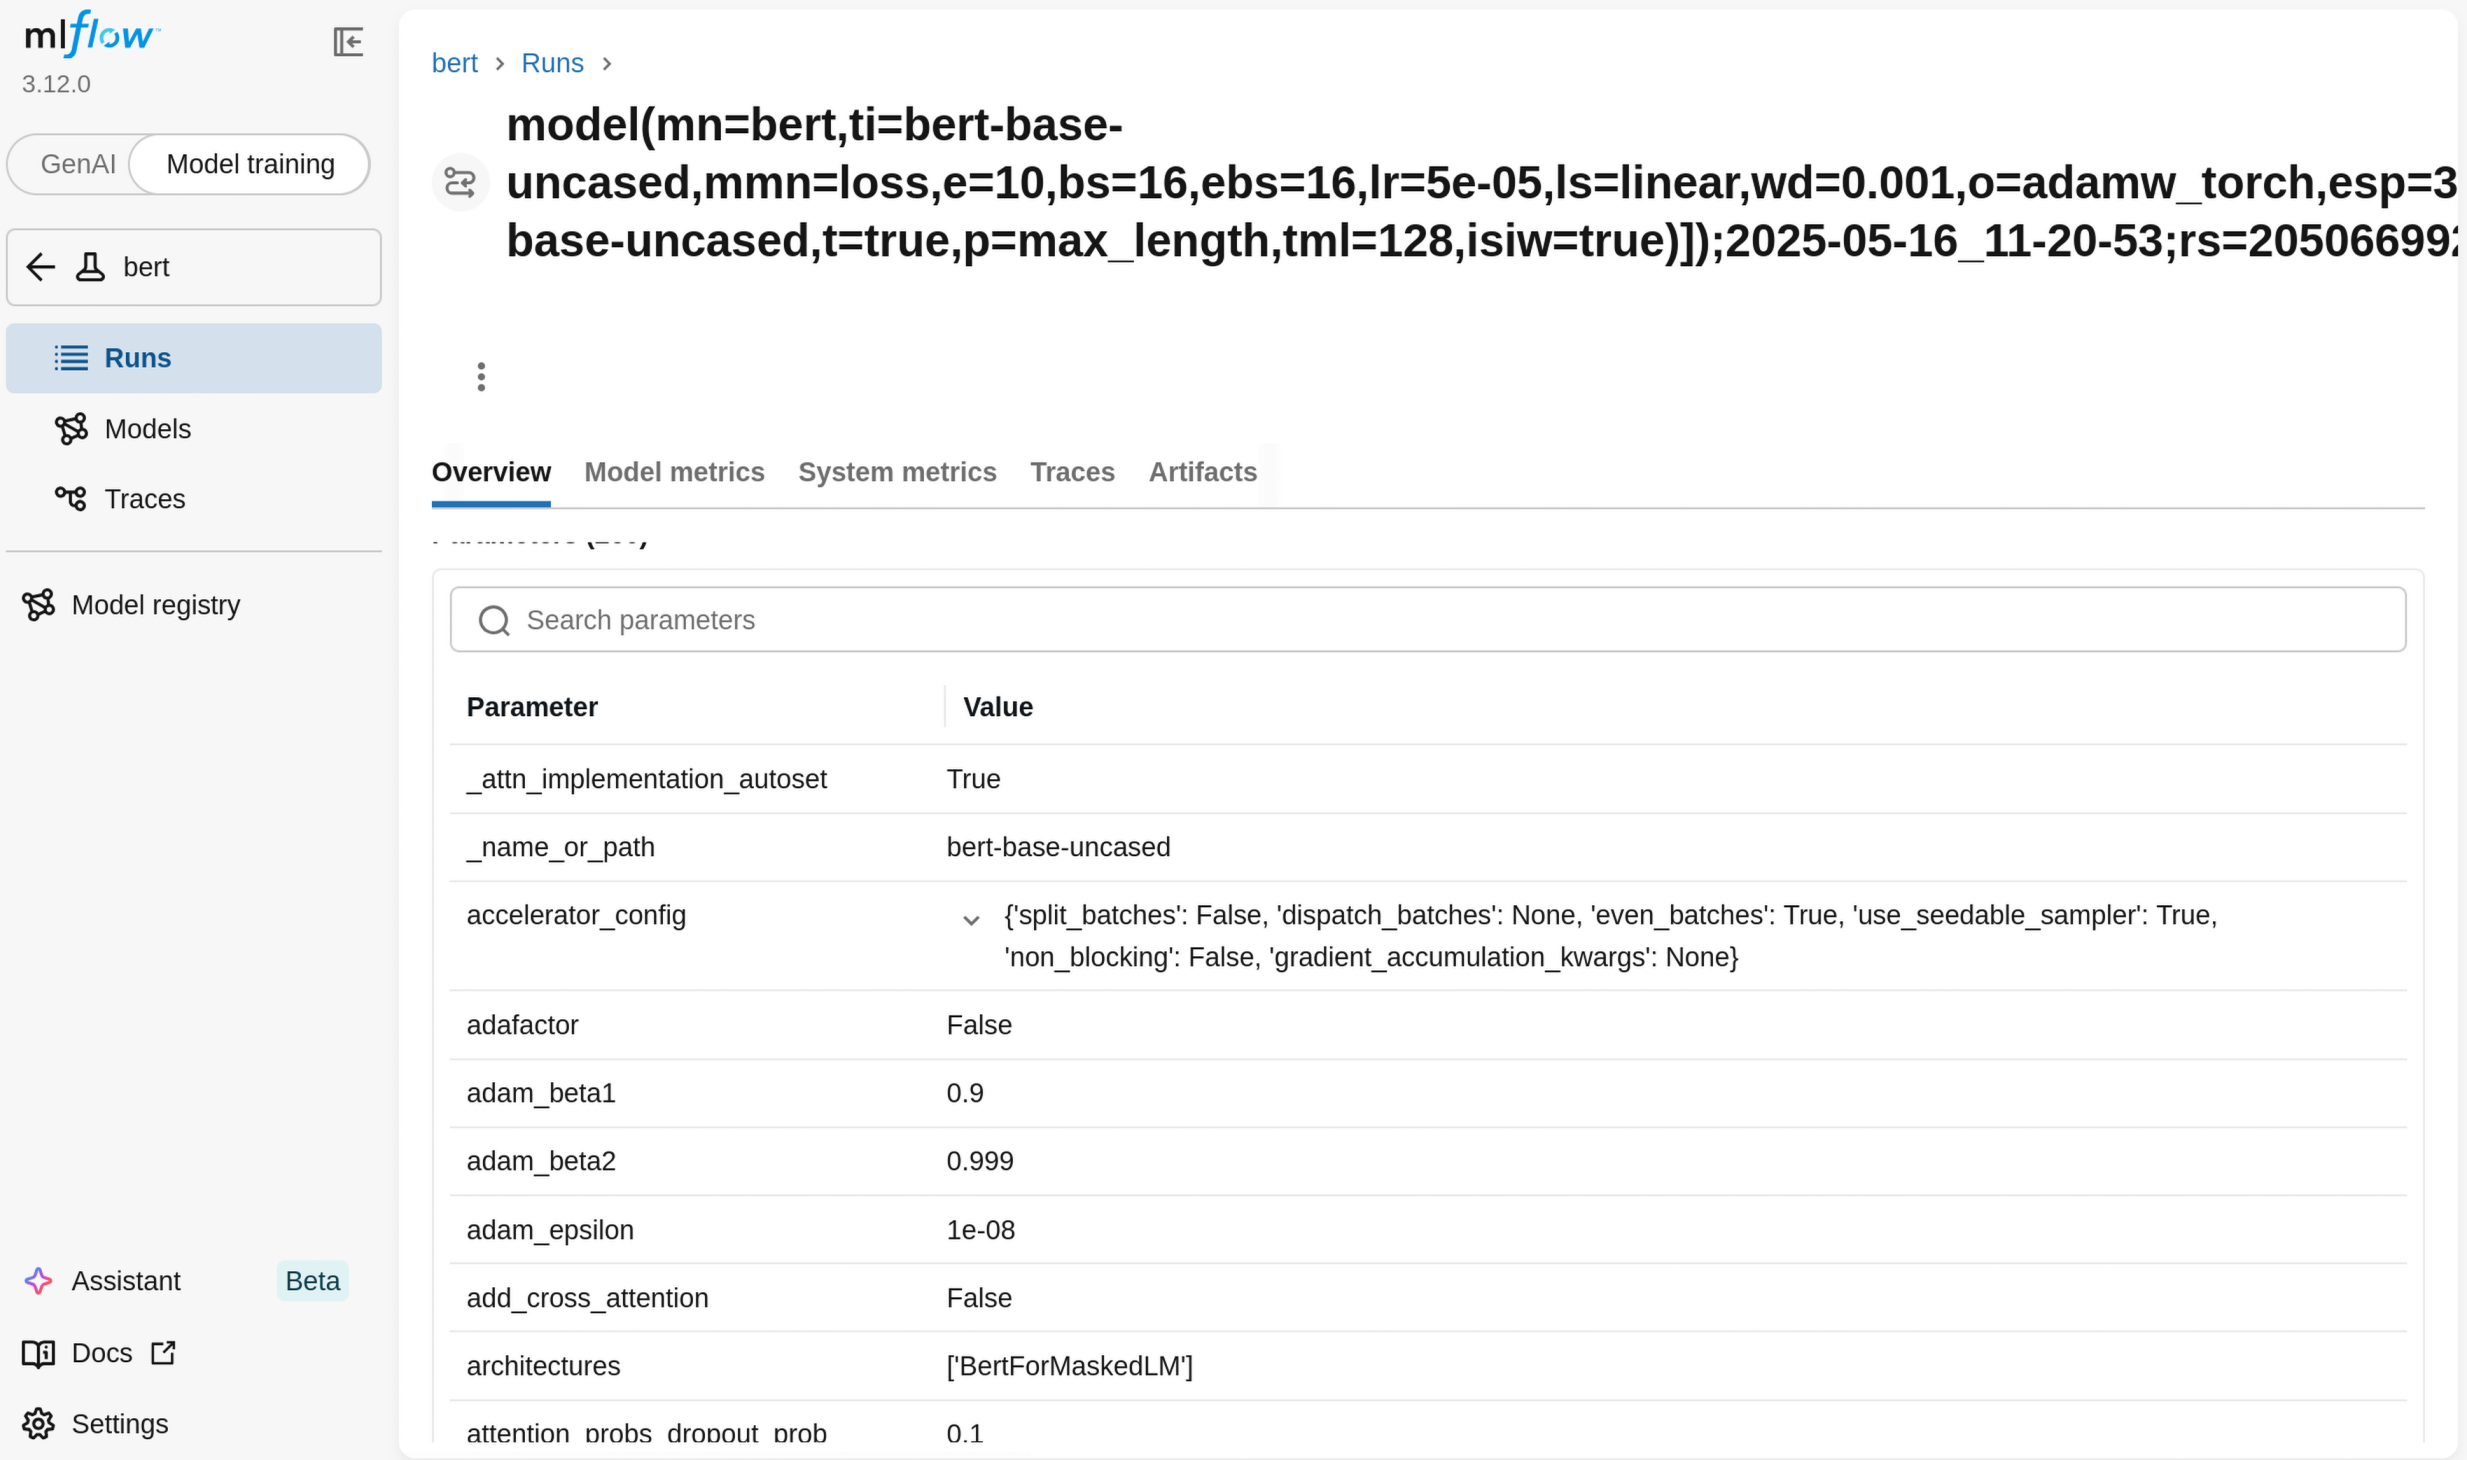
\includegraphics[width=\textwidth]{assets/mlflow_bert_run_details.png}
    \caption{Detailed information recorded for a single MLflow run}
    \label{fig:mlflow_bert_run_details}
\end{figure}

\FloatBarrier

\begin{markdown}

MLflow also supports artifacts storage, including trained model checkpoints and intermediate preprocessing outputs. During experimentation, this functionality proved useful for debugging preprocessing pipelines and verifying correct data ingestion into the models. The ability to inspect intermediate artifacts and recorded metrics significantly simplified the debugging process and improved the overall reliability of the experimental workflow.

\end{markdown}

\section{Experiments}

\begin{markdown}

This section describes the experimental workflow used in this thesis, including the training procedure, preprocessing pipeline configuration, and evaluation methodology.

\end{markdown}

\subsection{Training}

\begin{markdown}

The training pipeline was implemented using the Hugging Face Transformers framework together with PyTorch. The implementation relies primarily on the standard model and trainer abstractions provided by the framework, while extending them with additional functionality related to experiment logging and artifact tracking through MLflow.

The developed implementation is designed in a modular manner using abstract interfaces, allowing different preprocessing pipelines, models, and training configurations to be integrated into a unified experimental workflow.

Before training, a preprocessing pipeline is configured for each experimental run. The pipeline determines which preprocessing techniques are applied to the dataset before tokenization and model training.

\end{markdown}

\begin{lstlisting}[language=Python, basicstyle=\ttfamily\tiny]
# Example of preprocessing pipeline configuration for a training run

pipeline = PreprocessingPipeline(
    name='noise_reduction_with_stemming',
    iterable=[
        NoiseReduction(),
        NLTKTokenizer(),
        Stemming(),
        Encoder(
            is_split_into_words=True,
            truncation_max_length=max_tokens
        )
    ]
)
\end{lstlisting}

\begin{markdown}

Each preprocessing step automatically stores intermediate artifacts in MLflow, making it possible to inspect preprocessing outputs and verify the correctness of the pipeline during experimentation.

After preprocessing and tokenization, the encoded datasets are passed to the transformer training framework. Since the overall training procedure follows the standard workflow provided by the Transformers library, the complete implementation details are omitted.

As discussed in the dataset analysis chapter, transformer models in this work process a maximum of 512 tokens per sample. Any remaining tokens exceeding this limit are truncated and are therefore not included during training or inference.

Regarding dataset splitting, 70\% of the samples were used for training, 15\% for validation, and the remaining 15\% for testing. The validation set was used to monitor model performance during training and to select the best-performing checkpoint based on validation metrics. The selected checkpoint was then evaluated on the test set to obtain the final reported results.

\end{markdown}

\subsection{Evaluation}

\begin{markdown}

Evaluation of transformer-based architectures differs from the evaluation of simpler machine learning models because the models are trained over multiple epochs and their performance changes throughout the training process.

For each training run, evaluation metrics were recorded after every epoch. The final model checkpoint was selected according to the best validation accuracy achieved during training. In practice, this means that the checkpoint corresponding to the epoch with the highest validation accuracy was chosen as the final model for evaluation.

Several evaluation metrics were monitored during experimentation, including accuracy, precision, recall, F1-score, ROC-AUC, false positive rate, and false negative rate. Among these metrics, accuracy was selected as the primary comparison criterion in this thesis. This choice was made mainly to maintain consistency with the previous work by Jan Flajžík \cite{flajzik_classification_2024} and to simplify comparison between the classical and transformer-based approaches.

The selected checkpoint was subsequently evaluated on the test dataset to obtain the final reported results.

\end{markdown}

\section{Conclusion}

\begin{markdown}

One of the main contributions of this work is the implementation of a reusable and extensible experimental framework for transformer-based fake news classification. Training large neural architectures is computationally demanding and often requires extensive experimentation, making experiment tracking and reproducibility important aspects of the implementation.

Compared to the previous work by Jan Flajžík \cite{flajzik_classification_2024}, where most experiments were implemented directly in Jupyter notebooks, this thesis introduces a more modular software structure based on reusable Python modules. Jupyter notebooks were used primarily for hyperparameter exploration and interactive monitoring of ongoing experiments.

The integration of MLflow significantly simplified experiment management, debugging, and result analysis. The ability to store intermediate artifacts, preprocessing outputs, model checkpoints, and detailed training metrics proved particularly useful during debugging and validation of the experimental pipeline.

\end{markdown}